\nonstopmode
\documentclass[10pt, a4paper]{article}
\parindent=20pt
\parskip=8pt
\usepackage[width=15.5cm, left=3cm, top=2.5cm, height= 24.5cm]{geometry}
\usepackage[spanish]{babel}
\usepackage[utf8]{inputenc}
\usepackage{fancyhdr}
\usepackage{multirow}
\usepackage{rotating}
\usepackage{indentfirst}
\usepackage{latexsym}
\usepackage{caratula}
\usepackage{gnuplottex}
\usepackage{epsfig}
\usepackage{lastpage}
\usepackage{amsfonts}
\usepackage{listings}
\lstset{language=C}
%\usepackage[export]{adjustbox}
\usepackage{pdfpages}
\usepackage{amsmath}
\usepackage{verbatim}
%\usepackage[ruled,vlined,linesnumbered]{algorithm2e}
\usepackage{graphicx}
\usepackage{float}
\usepackage{color}

\graphicspath{{imgs/}}

% Acomodo fancyhdr.
\pagestyle{fancy}
\thispagestyle{fancy}
\addtolength{\headheight}{1pt}
\lhead{Teor\'ia de las Comunicaciones}
\rhead{TP1}
\cfoot{\thepage /\pageref{LastPage}}
\renewcommand{\footrulewidth}{0.4pt}
\renewcommand{\thesubsubsection}{\thesubsection.\alph{subsubsection}}


\author{Teor\'ia de las Comunicaciones, DC, UBA.}
\date{}
\title{}

\begin{document}
	
\thispagestyle{empty}
\materia{Teor\'ia de las Comunicaciones}
%\submateria{Trabajo Pr\'actico Nº1}
\titulo{Trabajo Práctico Nº2}
\integrante{Rivero, Maximiliano}{366/07}{maxirivero088@gmail.com}
\integrante{Izcovich, Sabrina}{550/11}{sizcovich@gmail.com}
\integrante{Rogani, Marcos}{520/05}{marcos.rogani@gmail.com}

\maketitle

\tableofcontents
\newpage

\section{Introducción}

%\begin{figure}[H] %[h] Aqui [b] para button [t] para top
%\begin{center}
%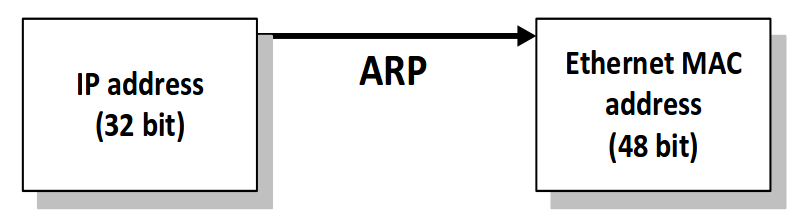
\includegraphics[width=250pt]{../imgs/IPtoMAC.png}
%\caption{Formato de una ARP.}
%\end{center}
%\end{figure}

\section{Desarrollo}


\section{Resultados}


\newpage
\section{Discusión}

\section{Conclusiones}


\section{Referencias}
\begin{itemize}
\item PETERSON, DAVIE ; Computer Networks, 5th edition, Wiley


\end{itemize}
\end{document}
